%!TEX root=ClassNotes.tex

\section{Integrals}
\subsection{Integrals as Areas}

\begin{figure}[H]
	\centering
	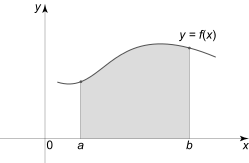
\includegraphics[width=0.5\textwidth]{integral.png}
	\caption*{Signed area under the curve is given by $\int_a^b f(t)\:dt$}
\end{figure}
The integral of a function captures the concept of an area.
\begin{align*}
	\int \limits_{a}^b f(t) dt = \mbox{ signed area between the curve $y=f(x)$ and the x-axis \strut}
\end{align*}
where by signed area we mean that the integral is negative if $f(x) < 0$ and hence equals negative of the area in this case (as area is always positive). This is a good {\it interpretation} but not a good {\it definition} as we have not rigorously defined what area is.
Instead we'll define the integral in terms of a limit and then define the (signed) area as the integral.

\begin{exercise}
	Express the following areas as (sums of) integrals. For each problem, draw pictures to justify your answer.
	\begin{enumerate}
		\item Area between the line $x + y = 1$, the x-axis and the y-axis.
		\item Area enclosed between the graph $y = \sin x$ and the x-axis for $x \in [0,2\pi]$.
		\item Area enclosed between the parabola $y=x^2$ and the line $y=1$.
		\item Area of a circle of radius 1.
	\end{enumerate}
\end{exercise}
Several physical quantities can be expressed as integrals, for example,
if $t$ denotes time and $f(t)$ is the speed of a particle then the integral measures the distance traveled, if $t$ denotes length and $f(t)$ is the linear density of a one dimensional object then the integral measures the total mass, etc.

\subsection{Definition of Integral}
We need several preliminary definitions to define the integral.
\begin{definition}$ $
	\begin{enumerate}
		\item For an interval $[a,b]$ a {\bf partition} $P$ is a sequence of real numbers
		      \begin{align*}
			      a = x_0 < x_1 < \dots < x_n = b
		      \end{align*}
		\item A {\bf uniform partition} $P_n$ of $[a,b]$ is the {\it uniform length} partition
		      \begin{align*}
			      x_0 & = a                          \\
			      x_1 & = a + \dfrac{b-a}{n}         \\
			          & \:\:\: \vdots                \\
			      x_i & = a + i \cdot \dfrac{b-a}{n} \\
			          & \:\:\: \vdots                \\
			      x_n & = b
		      \end{align*}
		\item For a partition $P$ define
		      \begin{align*}
			      M_i & = \sup \{ f(x) : x_i \le x \le x_{i+1}\} \\
			      m_i & = \inf \{ f(x) : x_i \le x \le x_{i+1}\}
		      \end{align*}
		      Define the {\bf upper Riemann sum} $U(f,P)$ and the {\bf lower Riemann sum} $L(f,P)$ as
		      \begin{align*}
			      U(f,P) & = \sum \limits_{i=0}^{n-1} M_i \cdot (x_{i+1} - x_i) \\
			      L(f,P) & = \sum \limits_{i=0}^{n-1} m_i \cdot (x_{i+1} - x_i)
		      \end{align*}
	\end{enumerate}
\end{definition}
\begin{figure}[H]
	\centering
	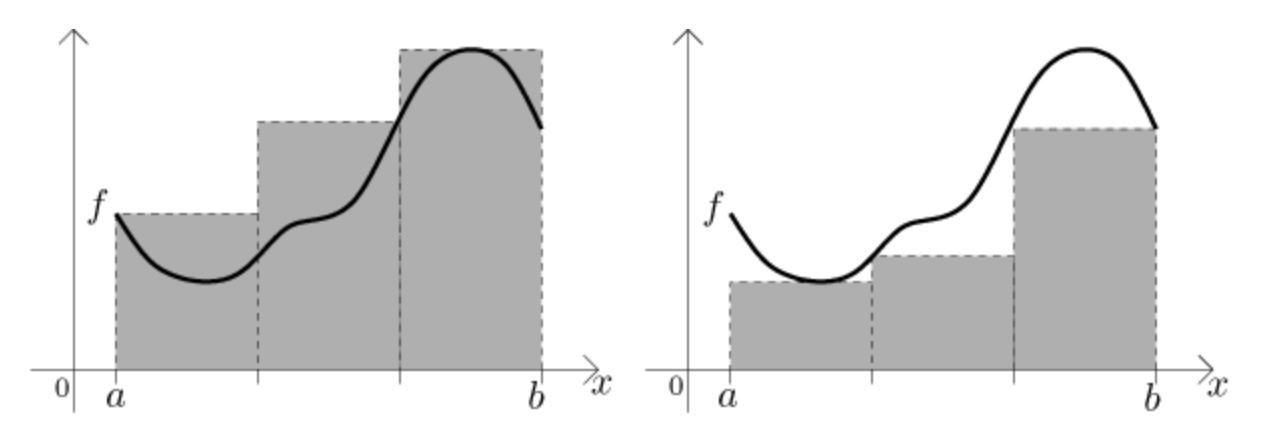
\includegraphics[width=0.8\textwidth]{RiemannSums2.png}
	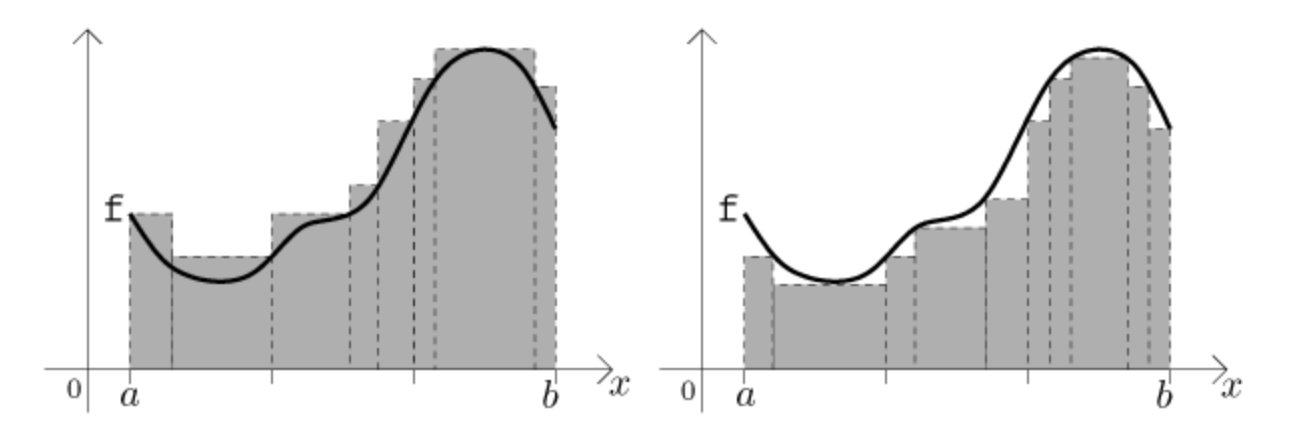
\includegraphics[width=0.8\textwidth]{RiemannSums1.png}
	\caption*{For finer partitions, the Riemann sums provide better approximations of the integral, hence in the limiting case as $n\rightarrow \infty$ we obtain the exact integral.}
\end{figure}
\begin{definition}
	\label{def:definition_Integral}
	We say that a function $f(x)$ is (Riemann) {\bf integrable} on an interval $[a,b]$ if there exists a real number $I$ such that
	\begin{align*}
		\lim \limits_{ n \rightarrow \infty} U(f,P_n) = I = \lim \limits_{ n \rightarrow \infty} L(f,P_n)
	\end{align*}
	In this case, we define the integral of $f$ on $[a,b]$ as
	\begin{align*}
		\int \limits_{a}^{b} f(t) \: dt & = I
	\end{align*}
\end{definition}
\noindent Thus when a function $f(x)$ is integrable it suffices to compute either $\lim \limits_{ n \rightarrow \infty} U(f,P_n)$ or $\lim \limits_{ n \rightarrow \infty} L(f,P_n)$ to compute the integral. \\

We'll assume the following theorem without proof. The proof requires the notion of {\bf uniform continuity} which is beyond the scope of this class.

\begin{theorem}
	\label{theorem:continuous_are_integrable}
	If $f$ is a continuous function on the interval $[a,b]$ then $f$ is integrable on $[a,b]$.
\end{theorem}

We'll do a few examples to better understand the definition of integral.
\begin{exercise}
	Let $f(x) = -x$, let $a=0$ and $b = 1$.
	\begin{enumerate}
		\item Use basic geometry to find $\int_{0}^1 f(t) \: dt$.
		\item Using pictures describe and compute $L(f,P_1)$, $L(f,P_2)$, and $L(f,P_3)$.
		\item Compute $L(f,P_n)$ where $n$ is a positive integer. You'll need to use
		      \begin{align*}
			      1 + 2 + 3 + \dots + n = \dfrac{n(n+1)}{2}
		      \end{align*}
		\item Find $\lim \limits_{n \rightarrow \infty} L(f,P_n)$, which equals $\int_{0}^1 f(t) \: dt$ by Theorem \ref{theorem:continuous_are_integrable}, and verify that it agrees with part 1.
	\end{enumerate}
\end{exercise}

\begin{exercise}
	Let $f(x) = x^2$, let $a=0$ and $b = 1$.
	\begin{enumerate}
		\item Compute $U(f,P_n)$ where $n$ is a positive integer. You'll need to use the identity
		      \begin{align*}
			      1^2 + 2^2 + 3^2 + \dots + n^2 = \dfrac{n(n+1)(2n+1)}{6}
		      \end{align*}
		\item Find $\lim \limits_{n \rightarrow \infty} U(f,P_n)$, which equals $\int_{0}^1 f(t) \: dt$ by Theorem \ref{theorem:continuous_are_integrable}.
	\end{enumerate}
\end{exercise}

\begin{exercise}
	Let $a = 0$, $b = 1$, and let
	\begin{align*}
		f(x) = \begin{cases}
			1 & \mbox{ if $x$ is rational}    \\
			0 & \mbox{ if $x$ is irrational.}
		\end{cases}
	\end{align*}
	\begin{enumerate}
		\item For $n$ a positive integer, compute $U(f,P_n)$ and $L(f,P_n)$.
		\item Find $\lim \limits_{n \rightarrow \infty} U(f,P_n)$ and $\lim \limits_{n \rightarrow \infty} L(f,P_n)$ and show that the $f(x)$ is not integrable.
	\end{enumerate}
\end{exercise}



\subsubsection{Indefinite Integrals}
We'll assume the following theorem without proof.
\begin{theorem}
	\label{theorem:integral_sum}
	For real numbers $a < b < c$, if $f$ is integrable on $[a,c]$ then
	\begin{align*}
		\int \limits_a ^c f(t) \: dt = \int \limits_a ^b f(t) \: dt  + \int \limits_b ^c f(t) \: dt
	\end{align*}
\end{theorem}
\begin{exercise}
	Draw a picture to explain the statement of the above theorem.
\end{exercise}

So far, we've only defined $\int_a^b f(t) \: dt$ for $a < b$. We now extend this to all real numbers $a$, $b$ by defining
\begin{align*}
	\int \limits_a^a f(t) \:dt
	= 0
	 &  & \mbox{ and } &  &
	\int \limits_a^b f(t) \:dt
	= -\int \limits_b^a f(t) \:dt
	\mbox{ \quad if } a > b
\end{align*}
With this extended notation one can check that Theorem \ref{theorem:integral_sum} is true for all real numbers $a$, $b$, $c$. For example, for $ a < b < c$
\begin{align*}
	         &  &
	\int \limits_a ^c f(t) \: dt = \int \limits_a ^b f(t) \: dt  + \int \limits_b ^c f(t) \: dt \\
	\implies &  &
	\int \limits_a ^c f(t) \: dt = \int \limits_a ^b f(t) \: dt  - \int \limits_c ^b f(t) \: dt \\
	\implies &  &
	\int \limits_a ^c f(t) \: dt + \int \limits_c ^b f(t) \: dt = \int \limits_a ^b f(t) \: dt
\end{align*}


\begin{definition}
	For an integrable function $f$ and a real number $a$, an {\bf antiderivative} is a function on the real numbers defined as
	\begin{align*}
		F_a(x) = \int \limits_a^x f(t) \: dt
	\end{align*}
\end{definition}

\begin{exercise}
	\label{q:difference_antiderivatives}
	For real numbers $a$, $b$ show that
	\begin{align*}
		F_a(x) - F_b(x)
	\end{align*}
	is a constant that does not depend on $x$.
\end{exercise}

Thus for any integrable function $f$ any two antiderivatives differ by a constant. This allows us to {\it define} the {\bf indefinite integral} denoted
\begin{align*}
	\int f(x) \: dx
\end{align*}
as $\int_a^x f(t) \: dt$ for some real number $a$. Changing the constant $a$ changes $F_a(x)$ by a constant, hence the indefinite integral is only defined up to a constant.
